\documentclass[class=book, crop=false, oneside]{standalone}
\usepackage[subpreambles=true]{standalone}

\usepackage{../../style}
\usepackage{../../set-citations}

\graphicspath{{./assets/images/}}

% arara: pdflatex: { synctex: yes, shell: yes }
% arara: latexmk: { clean: partial }
\begin{document}
\chapter{La gerarchia di memoria}\begin{fquote}[Burks, Goldstine, Von Neumann][1946]Idealmente si desidererebbe una memoria indefinitamente grande, in cui ogni particolare parola risulti immediatamente disponibile.
 \end{fquote}

\section{Introduzione}
Sottolineare quanto il concetto di memoria sia importante e necessario nei dispositivi elettronici del giorno d'oggi risulta abbastanza scontato. D'altra parte, viene fatta subito una precisazione: non esiste un'unica soluzione che permette di ottenere la memoria "perfetta". Esistono infatti diverse implementazioni, ognuna con i suoi compromessi, che variano per costo, prestazioni e capacità.

\section*{Qualche definizione}
Possiamo distinguere principalmente due tipologie di memoria in base alla modalità di accesso:
\begin{itemize}
	\item \emph{memoria indirizzata direttamente} (memoria principale, memoria cache):
	\begin{itemize}
		\item è volatile, ossia il suo contenuto viene perso se viene spento il calcolatore;
		\item è limitata per capacità dallo spazio di indirizzamento definito dall'architettura del processore;
		\item i dati contenuti nella memoria principale sono disponibili in qualsiasi momento;
	\end{itemize}
	\item \emph{memoria indirizzata indirettamente} (memoria periferica):
	\begin{itemize}
		\item è di tipo permanente, ossia mantiene il suo contenuto anche senza alimentazione;
		\item ha uno spazio di indirizzamento software che non dipende dall'architettura del processore;
		\item i dati contenuti nella memoria periferica devono essere trasferiti alla memoria principale prima di essere utilizzati (solitamente questo processo viene mediato dal software, tipicamente il sistema operativo);
	\end{itemize}
\end{itemize}

A seguire un elenco di definizioni che utilizzeremo in seguito.
\begin{itemize}
	\item \emph{Tempo di accesso}: è il tempo richiesto per \emph{una} operazione di lettura / scrittura nella memoria;
	\item \emph{Tempo di ciclo}: è il tempo che intercorre fra l'inizio di due istruzioni consecutive; è composto dal tempo di accesso sommato al tempo per muovere il dato con cui si stava lavorando;
	\item \emph{Latenza}: è il tempo di acceso ad una singola parola; indica quanto il processore dovrebbe poter aspettare un dato dalla memoria nel caso peggiore;
	\item \emph{Velocità o "banda"}: velocità di trasferimento massima in FPM; oltre ad essere importante per le operazioni FPM che sono legate all'utilizzo della memoria cache interne ai processori, è significativa per le operazioni in DMA (ossia quando un dispositivo periferico viene collegato alla memoria senza passare per il processore);
	\item \emph{Accesso casuale}: è quella modalità di accesso in cui non vi è alcun ordine o relazione fra i dati memorizzati; è tipico delle memorie a semiconduttori;
	\item \emph{Accesso sequenziale}: è quella modalità che presuppone lo scorrimento ordinato di un blocco di dati per accere ad un suo dato; il tempo d'accesso dipende dalla posizione fisica del dato nel supporto (tipicamente nastri e dischi);
	\item \emph{RAM} (\emph{Random Access Memory}): è una memoria dotata di accesso casuale che permette scrittura e lettura; viene implementata attraverso semiconduttori;
	\item \emph{ROM} (\emph{Read Only Memory}): è una memoria a semiconduttori che prevede solo un accesso in lettura; esistono implementazioni sia attraverso accesso casuale che sequenziale
\end{itemize}

\section{La memoria principale}
\subsection{Le RAM}
Con la seguente immagine descriviamo come avviene la connessione logica fra memoria RAM e CPU:
\begin{figure}[H]
	\centering
	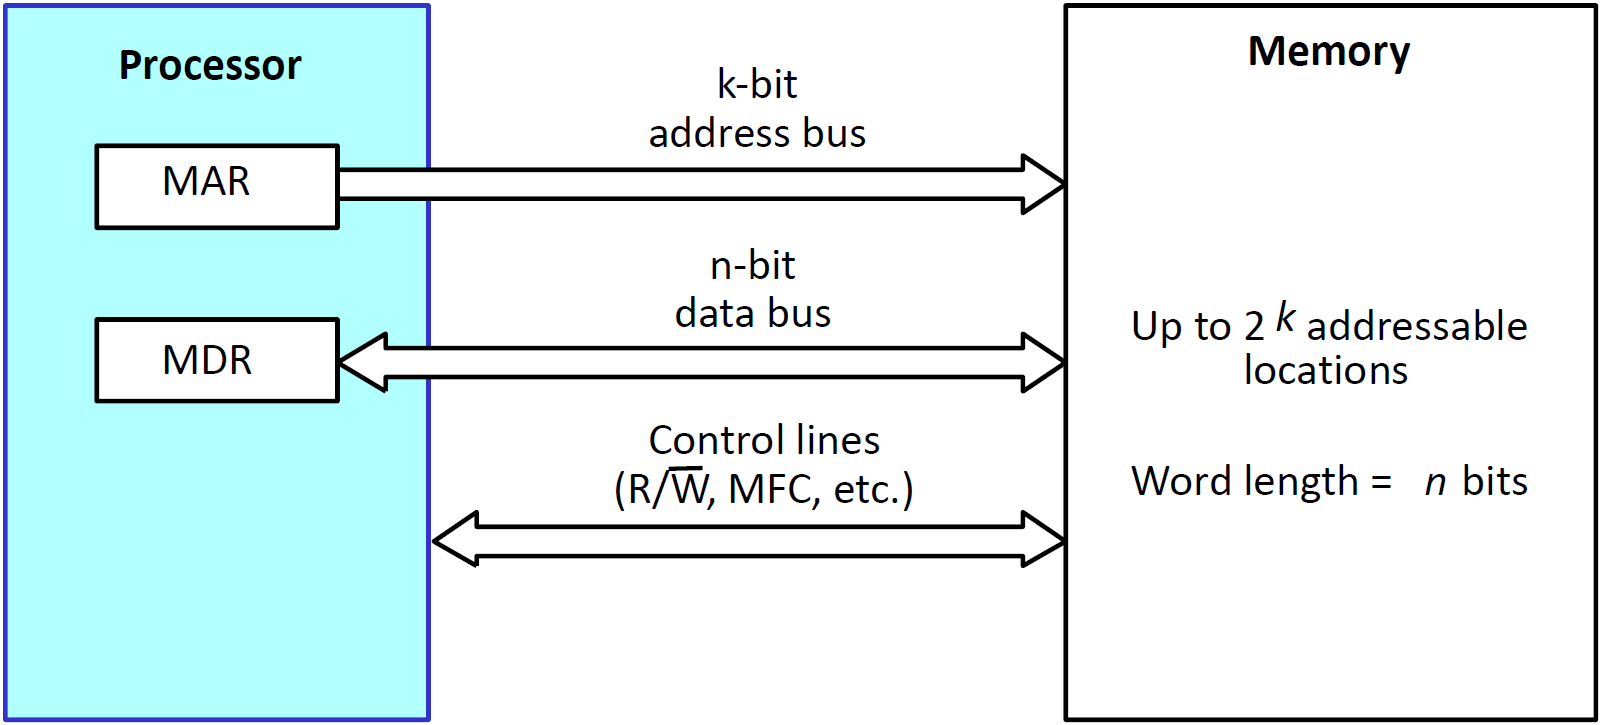
\includegraphics[width=\textwidth,keepaspectratio]{relazione_cpu_ram.png}
	\caption{Modello della relazioni logiche fra CPU e RAM}
\end{figure}
Esistono principalmente 3 bus che permettono di far comunicare il processore con la memoria:
\begin{itemize}
	\item \emph{MAR} (\emph{Memory Address Register}): è un bus a \(k\) bit, dove \(2^k\) sono il numero massimo di indirizzi accessibili direttamente in memoria. Dal punto di vista pratico contiene l'indirizzo del dato (o istruzione) che si vuole caricare o scrivere;
	\item \emph{MDR} (\emph{Memory Data Register}): è un bus a \(n\) bit, dove \(n\) è la lunghezza delle word nella memoria. Dal punto di vista pratico contiene il dato (o l'istruzione) che si vuole caricare o scrivere;
	\item \emph{bus di controllo:} è un bus che contiene vari codici di controllo che permettono di pilotare le relazioni fra memoria e CPU. Alcune linee di controllo sono: il bit \emph{MFC} (\emph{Memory Function Completed}) che permette di stabilire se l'operazione di lettura o scrittura è stata completata e il bit \emph{\(\textrm{R/}\overline{W}\)}, che distingue se si sta eseguendo un'operazione di lettura o scrittura.
\end{itemize}
Si noti che il \emph{MAR} è stato rappresentato da una freccia unidirezionale: dopo aver definito l'indirizzo di memoria su cui lavorare, infatti il processore non si aspetta il risultato. Vengono gestiti diversamente i bus di controllo e \emph{MDR}, i quali sono rappresentati con una freccia bidirezionale, in quanto sia la memoria che la CPU possono occupare il ruolo di mittente del messaggio.

Una memoria \emph{RAM} a semiconduttori principalmente memorizza singoli bit, memorizzati normalmente in gruppi di byte e/o word per motivi di efficienza. La memoria non necessariamente deve essere strutturata singolarmente: è possibile che sia suddivisa in diversi blocchi, al fine di favorire il parallelismo (si noti comunque che la dimensione complessiva della memoria non varia se presa in un unico blocco o se separata. Si ricorda che l'organizzazione di una memoria influenza il numero di pin di I/O del circuito integrato: più saranno, più aumenterà il costo.

\subsubsection{Organizzazione dei bit in un banco di memoria 16x8}
\begin{figure}[H]
	\centering
	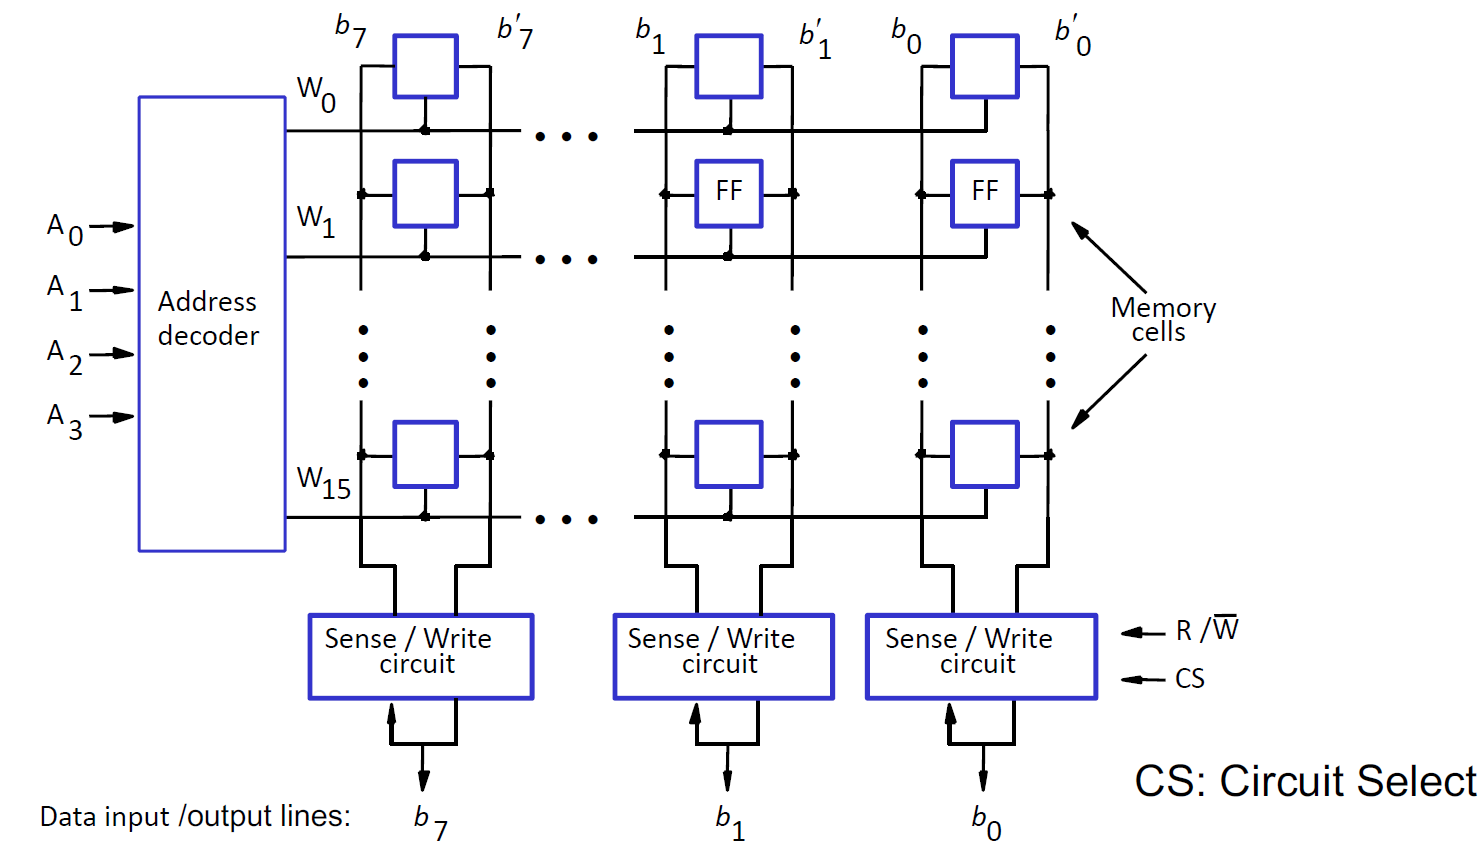
\includegraphics[width=\textwidth,keepaspectratio]{organizzazione.png}
	\caption{Organizzazione di un banco di memoria 16x8}
\end{figure}
Il caso presentato descrive il funzionamento di un banco di memoria formato da 16 righe e 8 colonne, con celle da un byte ciascuna. Si noti che per indirizzare un certo elemento all'interno della matrice del banco di memoria è necessario attivare una determinata riga e colonna (come avverrebbe in battaglia navale). Analizziamo ora, in ordine temporale, le operazioni che permettono di accedere/scrivere un determinato dato.
\begin{enumerate}
	\item In base alla riga da selezionare, l'\emph{address decoder} genera un 1 nell'uscita della riga corrispondente;
	\item Avviene un meccanismo simile anche per le colonne, attraverso il \emph{circuit select}, che decide se abilitare ciascuna colonna;
	\item Ogni colonna è gestita da un \emph{Sense/Write circuit} che riceve in input due linee di controllo: una definisce se eseguire l'operazione di lettura o scrittura (\emph{\(\textrm{R/}\overline{W}\)}) mentre l'altra (\emph{CS}) definisce se attivare o meno la colonna. Nel caso di una read, legge il valore contenuto nel bus della colonna (1 byte nel nostro esempio), altrimenti, nel caso di write, fa circolare il valore che si vuole scrivere nel bus della colonna. Per avere certezza dell'integrità dei dati, viene propagato sia il dato stesso che si vuole scrivere, che il suo negato. Ad esempio, nella colonna 0, \(b_0\) contiene il dato asserito, mentre \(b'_0\) contiene il dato negato;
	\item In base a com'è stata implementata la memoria (\emph{SRAM} o \emph{DRAM}), viene attivata la cella selezionata dalla colonna e dalla riga designata: su di essa verrà eseguita l'operazione di lettura/scrittura richiesta.
\end{enumerate}

Nelle prossime sezioni affronteremo come varia l'implementazione di ciascuna cella di memoria da \emph{SRAM} a \emph{DRAM}.

\subsection{Le SRAM}
Le \emph{SRAM}, ossia le RAM statiche, sono delle memorie in cui i bit possono essere mantenuti indefinitivamente (posto il fatto che non manchi l'alimentazione). Seppur abbiano tempi di accesso molto ridotti (nell'ordine di pochi nanosecondi) e consumino poca corrente, il loro costo è molto elevato: per ciascuna cella di memorizzazione vengono impiegati molteplici componenti.
Il funzionamento che sta alla base di una cella di SRAM è quello del flip flop (in particolare ai latch tipo D).

\begin{figure}[H]
	\centering
	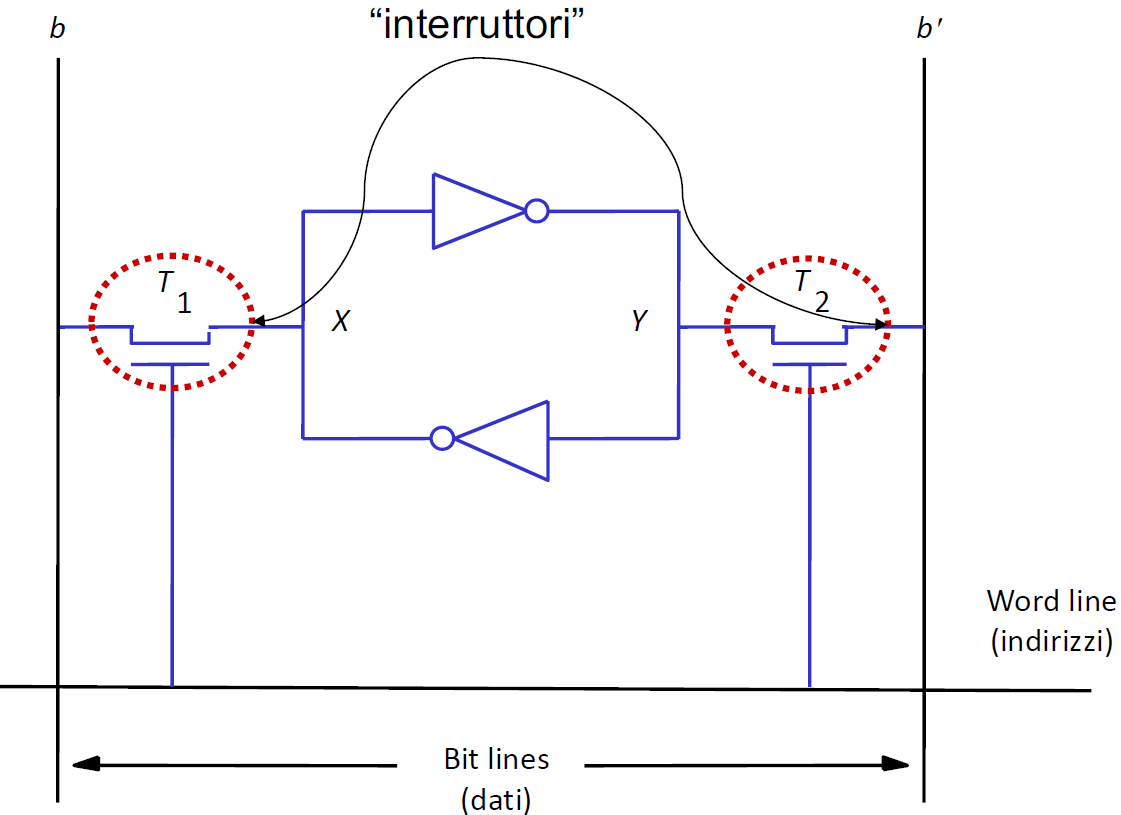
\includegraphics[width=\textwidth,keepaspectratio]{cella_SRAM.png}
	\caption{SRAM: memorizzazione di un bit}
\end{figure}

Nell'immagine, \(\textrm{T}_1\) e \(\textrm{T}_2\) sono due transistor\footnote{Attraverso gli ultimi ritrovati dell'ingeneria, è possibile realizzare dei transistor nell'ordine di grandezza dei nanometri}: in base al variare della tensione nel loro \emph{gate} (ossia il collegamento inferiore) permettono o meno il passaggio di corrente fra i rami laterali. Il funzionamento ricorda molto quello di un interruttore: se il gate ha ua tensione pari a Vdd, allora il circuito viene chiuso, altrimenti rimane aperto. Si noti che se la linea della word è bassa, allora gli interruttori \(\textrm{T}_1\) e \(\textrm{T}_2\) sono aperti: il consumo è praticamente nullo.\\
Dunque, nel caso venga chiuso il circuito, è possibile effettuare delle operazioni di lettura e di scrittura (gestite dal \emph{Sense/Write circuit}). Invece, nel caso in cui il circuito venisse aperto, la corrente circola solamente all'interno del latch a doppio NOT. La presenza di due NOT, permette di rinforzare il risultato e ridurre il tasso di errore, in quanto si vuole controllare la coerenza delle informazioni sia col segnale \emph{b} che col segnale \emph{b'} (si ricorda che \emph{b} contiene il segnale asserito, mentre \emph{b'} contiene il segnale negato: \emph{b}\(= NOT\)\emph{b'}).

\subsection{Le DRAM}
Le \emph{DRAM}, ossia le RAM dinamiche, sono le memorie più diffuse nei computer. Sono dotate di costi molto contenuti e di un'elevatissima densità, dovuta al fatto di dover impiegare un solo componente per ogni singola cella di memoria. Il concetto che sta alla base della DRAM è un circuito RC (la resistenza è quella data dal filo): la capacità di memorizzazione viene ottenuta attraverso la carica di un condensatore. Presentano però un difetto, che comporta consumi molto elevati: la cella di memoria necessita di un refresh continuo, altrimenti il proprio contenuto svanisce a causa delle correnti parassite.

\begin{figure}[H]
	\centering
	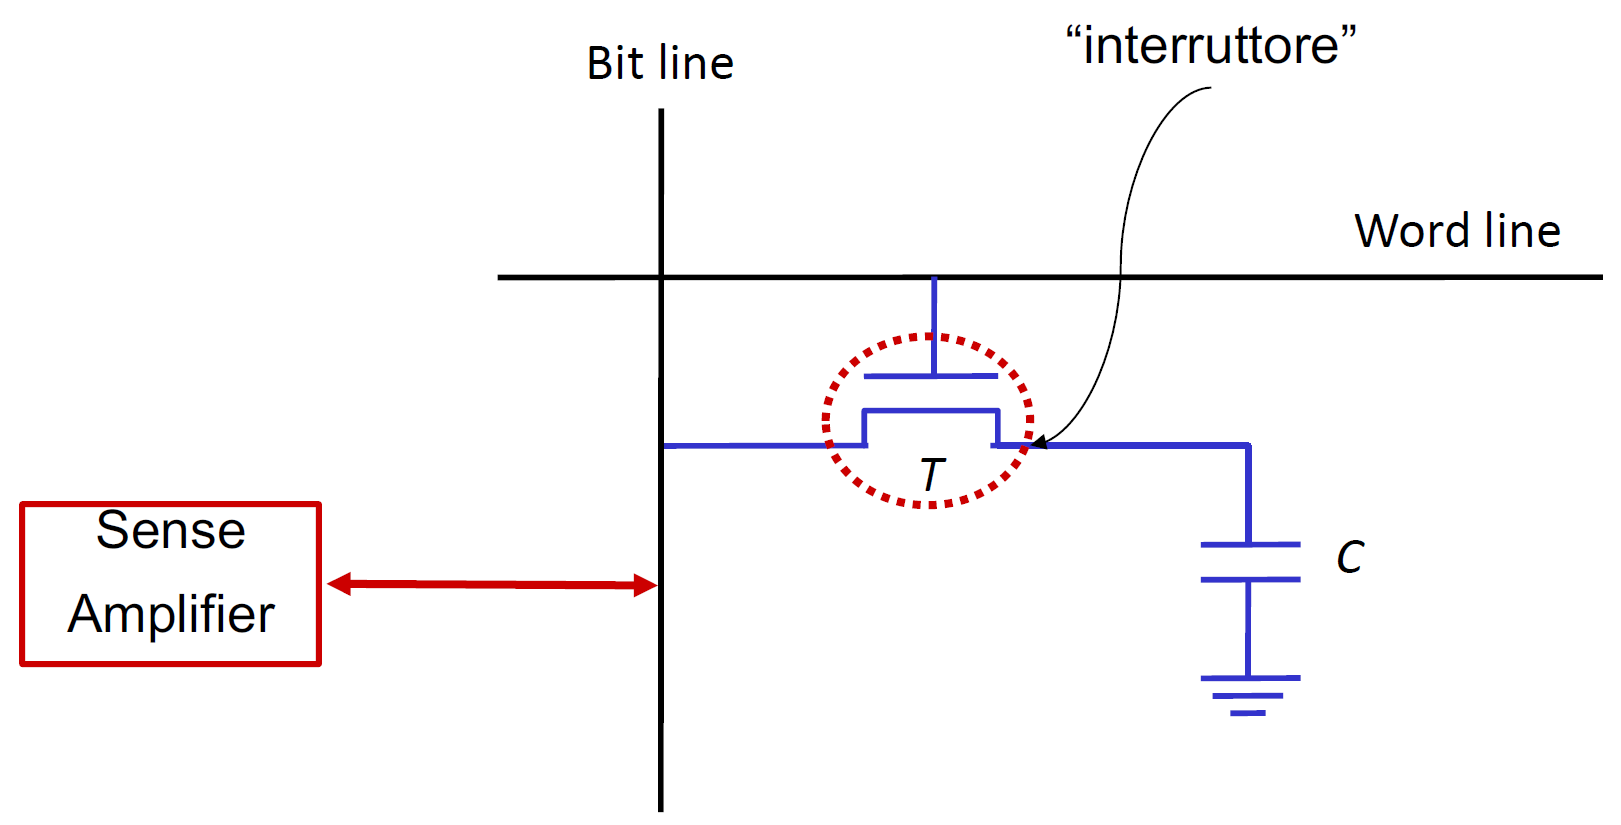
\includegraphics[width=\textwidth,keepaspectratio]{cella_DRAM.png}
	\caption{DRAM: memorizzazione di un bit}
\end{figure}

Nell'immagine \(\textrm{T}\) è un transistor: svolge una funzione di interruttore, in quanto permette collegare o meno il circuito RC alla bit line e alla word line. Se il circuito viene chiuso il condensatore viene caricato, altrimenti si scarica (ricordiamo che il processo di carica/scarica di un condensatore è esponenziale). Si ricorda che se non viene attivata la bit line o la word line, allora il circuito RC è scollegato, con la conseguente scarica del condensatore a causa della resistenza applicata. Dunque, se si vuole mantenere in memoria il dato 1, c'è la necessità di continuare a scrivere 1 nella cella di memoria ad ogni intervallo \(t_0\), altrimenti la scarica del condensatore annullerebbe il valore. Se il valore che si vuole memorizzare è 0, basta semplicemente lasciare disattivato il circuito (attenzione ad avergli lasciato il tempo necessario affinché si scarichi). Dunque per "refreshare" la memoria basta fare un ciclo di lettura: questo processo viene eseguito da un circuito di refresh, in maniera tale che l'utente non si debba programmare di questo meccanismo.

Solitamente si può considerare un condensatore scarico nel momento in cui la tensione ai suoi capi è inferiore a \(\frac{\textrm{Vdd}}{2}\). Vediamo nelle seguenti immagini dei grafici di carica e scarica del consensatore.

% TODO grafici di carica e scarica del condensatore

\subsubsection{La multiplazione dei indirizzi}
Facciamo un salto indietro di astrazione. L'immagine rappresenta l'organizzazione di una DRAM. A è l'indirizzo con cui si inidicizza un dato in memoria: dalla posizione 20 a 9 definisce il valore da dare in input al decoder delle righe, dalla posizione 8 alla 0 definisce il valore da dare al decoder delle colonne. Questa DRAM è caratterizzata da 4096 (\(2^{12}\), dove 12 rappresenta il numeri di bit di A per indirizzare la riga) righe e 512 (\(2^9\), dove 9 rappresenta il numero di bit di A per indirizzare la colonna) colonne:
\begin{figure}[H]
	\centering
	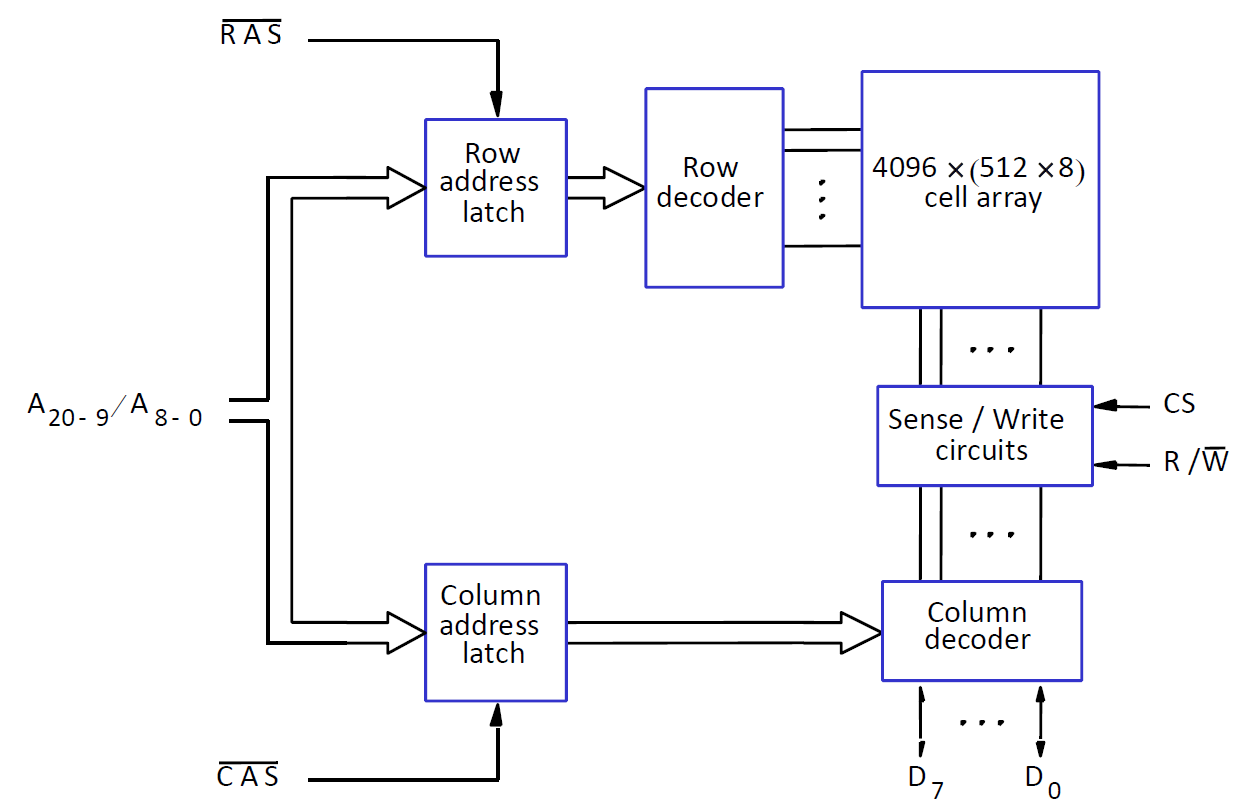
\includegraphics[width=\textwidth,keepaspectratio]{organizzazione_generale.png}
	\caption{Organizzazione generale di una memoria}
\end{figure}
Si noti che sono stati inseriti due circuiti: \emph{row address latch} e \emph{column address latch}, che rispettivamente ricevono in input i codici di controllo \emph{\(\overline{RAS}\)} e \emph{\(\overline{CAS}\)}. Queste due linee di controllo permettono di decidere, in base al loro input, se è possibile accedere ad una riga/colonna.

\subsubsection{Fast Page Mode (FPM)}
Solitamente i trasferimenti da/per la memoria avvengono a blocchi piuttosto che per singole celle. Ciò comporta un notevole risparmio di tempo, in quanto sarebbe necessario solo un unico indirizzamento per le righe e colonne. Questo processo viene chiamato \emph{fast page mode} (\emph{FPM}). Si sottolinea che questa modalità è del tutto automatica: l'utente non deve preoccuparsi di gestire questo meccanismo.

\subsubsection{Le DRAM sincrone}
Le DRAM che sono state descritte fin'ora sono dette \emph{asincrone}, in quanto non esiste una precisa temporizzazione di accesso: la dinamica viene governata dai segnali \emph{RAS} e \emph{CAS}. Si noti che questa asincronicità può causare non pochi problemi, soprattutto mentre si esegue il refresh della memoria. Una soluzione consiste nell'aggiungere dei buffer di memorizzazione degli ingressi e delle uscite, in maniera tale da riuscire a disaccoppiare la lettura e scrittura dal refresh della memoria, ottenendo automaticamente un accesso FPM pilotato dal clock. Questa implementazione della DRAM viene detta \emph{sincrona}. A seguire un'immagine che contiene uno schema riassuntivo:
\begin{figure}[H]
	\centering
	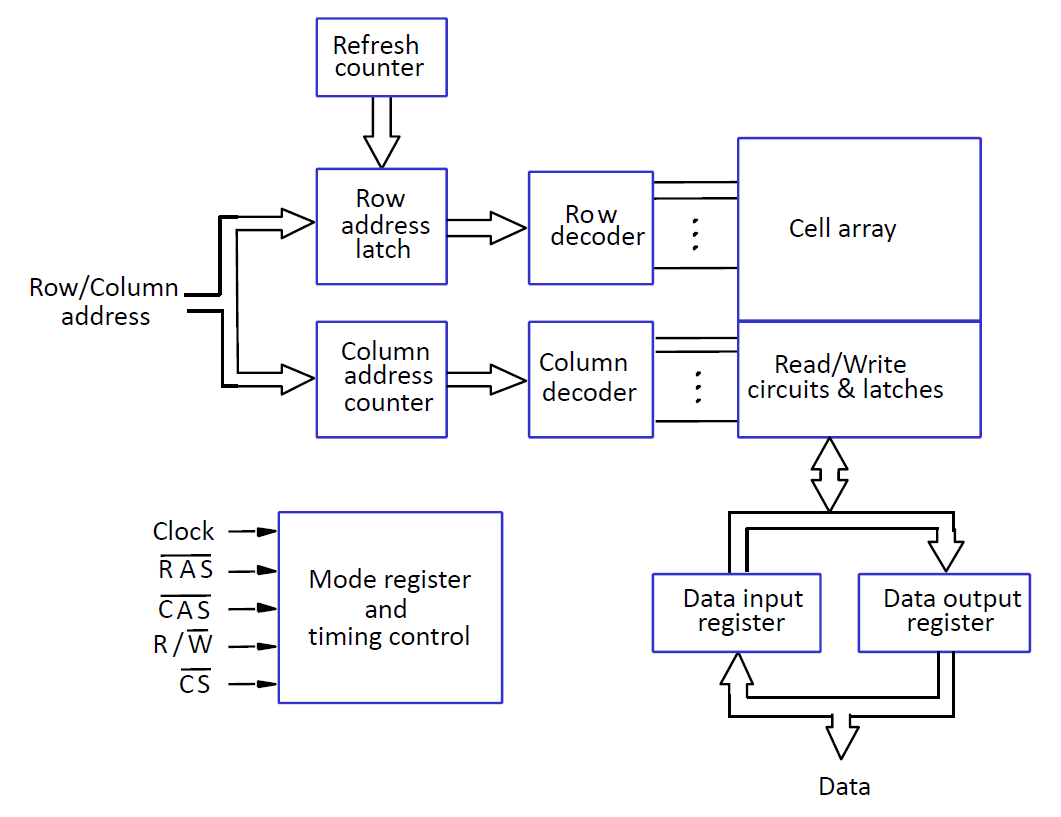
\includegraphics[width=\textwidth,keepaspectratio]{DRAM_sincrona.png}
	\caption{Organizzazione generale di una DRAM sincrona}
\end{figure}

Nella prossima immagine è possibile visualizzare un accesso sincrono in FPM:
\begin{figure}[H]
	\centering
	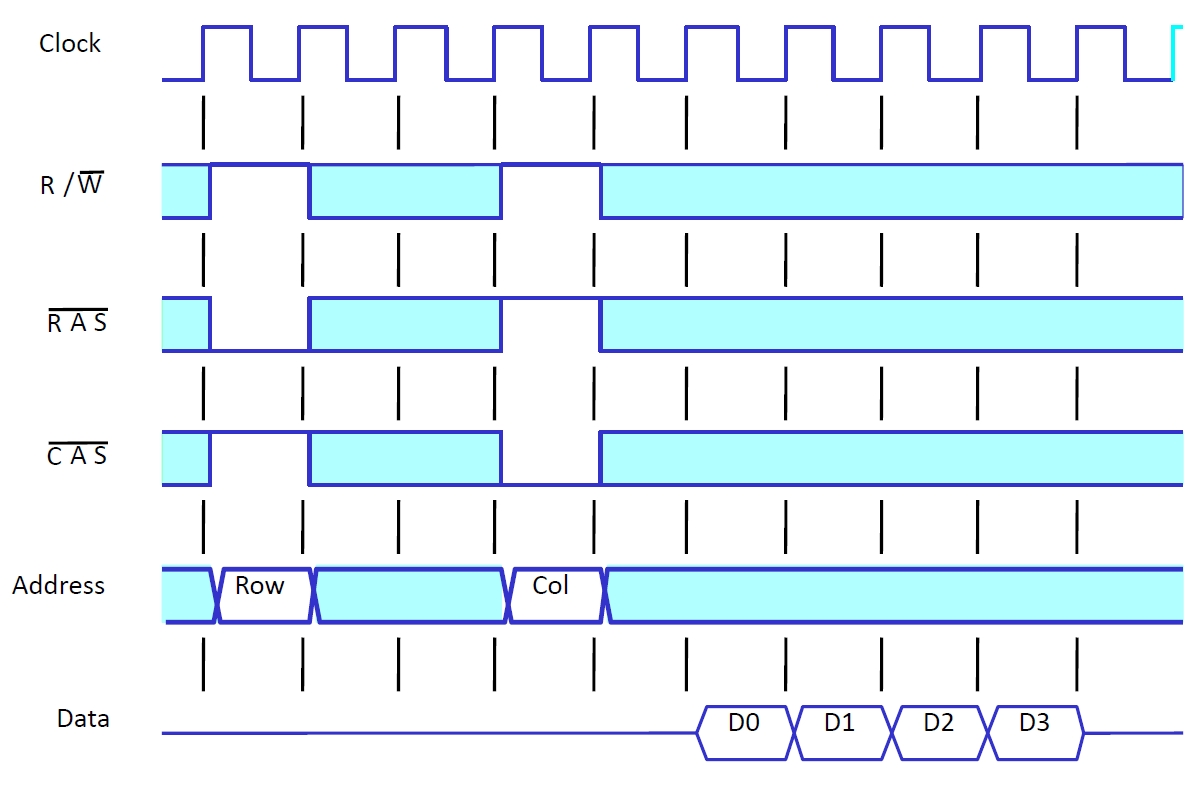
\includegraphics[width=\textwidth,keepaspectratio]{FPM.png}
	\caption{Funzionamento first page mode}
\end{figure}
dove il segnale di clock rappresentato è quello della memoria RAM: le operazioni di lettura e scrittura sono sincronizzate col fronte di salita; D0, D1, D2, D3 sono i byte che arrivano in serie; i valori rimanenti sono le linee di controllo.

\subsubsection{Double Data Rate SDRAM (DDR-SDRAM)}
Un ulteriore miglioramento è effettuato dalla \emph{DDR-SDRAM} (\emph{Double Data Rate SDRAM}): essa permette il trasferimento dei dati sia sul fronte di salita che sul fronte di discesa del clock della memoria. In poche parole ciò permette di raddoppiare le prestazioni rispetto ad una normale SDRAM: seppur la latenza rimane invariata, la banda viene raddoppiata.

Sono ottenute organizzando la memoria in due banchi separati: uno contiene le posizioni pari (a cui si accede durante il fronte di salita), l'altro contiene quelle dispari (a cui si accede durante il fronte di discesa). Locazioni contingue risultano divise fra i due banchi: grazie a qusto è possibile effettuare un accesso in modo interlacciato.


\end{document}
